% Template for PLoS
% Version 1.0 January 2009
%
% To compile to pdf, run:
% latex plos.template
% bibtex plos.template
% latex plos.template
% latex plos.template
% dvipdf plos.template

\documentclass[letterpaper,11pt]{article}

% amsmath package, useful for mathematical formulas
\usepackage{amsmath}
% amssymb package, useful for mathematical symbols
\usepackage{amssymb}

% graphicx package, useful for including eps and pdf graphics
% include graphics with the command \includegraphics
\usepackage{graphicx}

% cite package, to clean up citations in the main text. Do not remove.
\usepackage{cite}

\usepackage{color} 

% Use doublespacing - comment out for single spacing
%\usepackage{setspace} 
%\doublespacing


% Text layout
\usepackage[top=0.7in, bottom=0.65in, foot=0.7in, left=0.7in, right=0.7in]{geometry}
\usepackage[font={scriptsize}]{caption}
\usepackage[font={scriptsize}]{subcaption}
\usepackage{layout}
\usepackage{wrapfig}
\usepackage[scaled]{uarial}
\renewcommand*\familydefault{\sfdefault} 
\usepackage[T1]{fontenc}
%\usepackage{fontspec}
%\setmainfont{Arial}
\usepackage{fancyhdr}
\usepackage{wrapfig}
\setlength{\footskip}{20pt}
\setlength{\parskip}{.2\baselineskip}
\pagestyle{fancy}
\fancyhf{}
\renewcommand{\headrulewidth}{0.0pt}
\renewcommand{\footrulewidth}{0.0pt}
\lfoot{\footnotesize \textit{ GeoConvention 2015: New Horizons} }
\cfoot{}
\rfoot{\footnotesize \thepage}
\lhead{}
\chead{}
\rhead{}
\setlength\parindent{0pt}
\fancypagestyle{sty1}{
\fancyhf{}
\renewcommand{\headrulewidth}{0.0pt}
\renewcommand{\footrulewidth}{0.0pt}
\lfoot{\footnotesize \textit{ GeoConvention 2014: New Horizons} }
\cfoot{}
\rfoot{\footnotesize \thepage}
\lhead{}
\chead{}
\rhead{}
}
% Bold the 'Figure #' in the caption and separate it with a period
% Captions will be left justified
\usepackage[labelfont=bf,labelsep=period,justification=raggedright]{caption}
\usepackage{lipsum}
\usepackage{setspace}
\usepackage{titlesec}
\usepackage{natbib}
\usepackage{acro}
\usepackage{UsefulStuff}
\titlespacing\section{0pt}{0pt plus 0pt minus 0pt}{-0pt plus 2pt minus 2pt}
\titlespacing\subsection{0pt}{0pt plus 0pt minus 0pt}{-0pt plus 2pt minus 2pt}
\titlespacing\subsubsection{0pt}{0pt plus 0pt minus 0pt}{-0pt plus 2pt minus 2pt}
% Use the PLoS provided bibtex style
%\bibliographystyle{abbrv}
\frenchspacing
\linespread{0.95}
\begin{document}
%\thispagestyle{sty1}
\evg{what about using another font? that one is really old}
\begin{center}

\includegraphics[width=9.22cm]{header.png} \vspace{-1pt}
\end{center}

% Title must be 150 characters or less
\begin{flushleft}
{\LARGE
\begin{spacing}{0.9}
\textbf{Event origin depth uncertainty - estimation and mitigation using waveform similarity.}
\end{spacing}
}

% Insert Author names, affiliations and corresponding author email.
%\\
\textit{Anton Biryukov${}^1$, Evgenii Chzhen${}^2$, Jan Dettmer${}^1$, David Eaton${}^1$} \\
\textit{${}^1$ Department of Geoscience, University of Calgary, Calgary, AB, Canada} \\
\textit{${}^2$ LAMA, UMR-CNRS 8050, Universit\'{e} Paris Est -- Marne-la-Vall\'{e}e}
\end{flushleft}

\section*{Summary}
%
\evg{before: 5, after: $5$}
The induced seismicity event localization using inverse kinematic algorithms is still a problem requiring special attention. Often a catalog of events detected and located using limited on-surface instrumentation lacks the precision of origin depth. Such errors can hinder the interpretation of activated zones using seismicity as a proxy.

The location constraints are affected by the inaccuracy of the velocity model, limited acquisition geometry and the assumptions inherited by the location algorithm, among other factors. The issue becomes even more aggravated when only surface arrays are employed, where the geometry strongly favors the accuracy of epicentral location as opposed to depth location. The reported depth errors are sometimes comparable to a formation thickness or even the origin depth itself. The passive seismicity is often located using the P and S first breaks only. Finding additional features of the seismic signal that could be informative of its origin can be a first step towards constraining the depth uncertainty. 

Therefore, the purpose of this study was two-fold. First, we characterized the uncertainty in the event origin due to the inaccuracy in the effective velocity model using Monte-Carlo simulations. We show that a low velocity zone (\textsc{LVZ}) \evg{Harmonized abbriviations} can cause the non-uniqueness and a spread of the solution over a depth range. Subsequently, seismograms from a set of synthetic earthquakes were simulated spanning the depth range of $2-5$ km, covering \textsc{LVZ}. By varying the focal mechanism and event origin, we numerically generate a bank of waveforms corresponding to the events with known locations. A set of classifiers is trained on the bank to predict the event location with respect to \textsc{LVZ} based on arrival times and statistical features of the signal waveforms. We demonstrate that adding several features of the signal, descriptive of its origin can improve the location depth constraint, as opposed to using arrival times only as predictor variables.
%
\section*{Introduction}
The earthquake localization on a regional scale using inverse kinematic algorithms is still a problem requiring special attention. The on-surface seismic networks for monitoring induced seismicity provide a sufficient location accuracy for the earthquake hypocenter, but often offer very limited resolution in depth \citep{eisner_uncertainties_2009}. For computational convenience and due to the lack of information, the velocity model used for location is often parametrized as a function of depth only. In some cases such an approximation is a very strong assumption, and it is important to consider several different possible $1$D structures to test the sensitivity of the location to errors in the velocity model. The sparsely distributed on-surface instrumentation and insufficient azimuthal or vertical coverage can aggravate the location uncertainty due to the limited direction of the ray-paths it is able to receive \citep{eisner_comparison_2010}. As a result, in the absence of downhole observations, the reported uncertainty of the depth location using on-surface array only may be comparable to the origin depth value itself, such that the location of the event becomes untrustworthy to the analyst. On the other hand, in the daily industry practice the event origins are often derived based on the deterministic methods that use only $2$ characteristic points (P- and S-wave arrivals) per sensor per event. The information transmitted by the event is obviously not limited to two-points only, and therefore should not be discarded when the location is performed. Improving event location can be done through finding informative features of the seismic signal that could help better constrain the location. 


We start with a rigorous study of the effect of the uncertainty in the velocity model on the P- and S-wave travel time error. The ray-tracing method is employed to predict the time of the arrivals for the two phases at station location. The Monte-Carlo simulation is then performed with varying velocity model to estimate the mean and standard deviation of the arrival time. These values are consequently used as a proxy for an event's P- and S-wave arrival time uncertainties. Using non-linear location methods \citep{lomax_precise_2001}, the arrival times from the Monte-Carlo simulations can be translated into spatial uncertainties and thus give an error estimate due to uncertainty in the velocity model, given an event location.

Subsequently, we simulate the synthetic seismograms from the virtual sources spanning the depth range of $2-5$ km. A set of characteristic functions is applied to the resultant traces in order to extract features describing the origin. Later, a classification of the event location is carried out on two separate feature sets: (i) arrival times only and (ii) arrival times bundled with the signal features. With this comparison we highlight that the travel time data may be insufficient to constrain the origin of the event due to the velocity model accuracy while adding the waveform features has a potential to constrain the origin depth.

\section*{Methods}
\subsection*{Generalized workflow}
\begin{wrapfigure}{R}{0.3\textwidth}
\vspace{-4mm}
\centering
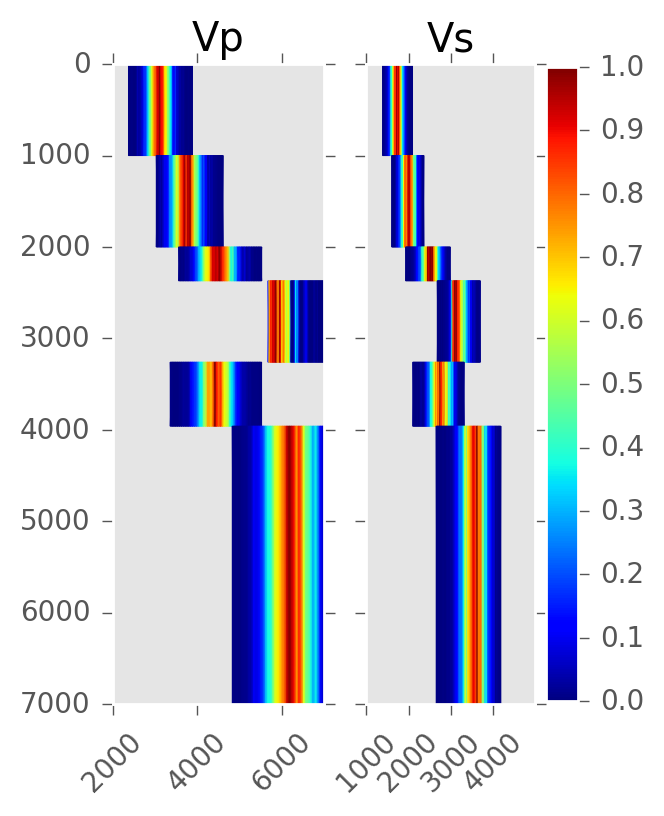
\includegraphics[width=0.28\textwidth]{./AntonBiryukov_bibtex/VpVs.png}
\vspace{-4mm}
\caption{An example of the distribution of velocity profile used in the MC simulations. The color represents the values of PDF of the velocity distribution. Note the limited variation of the layer above \textsc{LVZ} due to the creation of the shadow zone.}
\label{fig:vpvs}
\end{wrapfigure}
This report is particularly focused on estimating the depth error due to the velocity model uncertainty. That is, we want to evaluate the jitter in the hypocenter location due to inaccuracy in the approximation of the true velocity model as a 1D layered cake model derived from $V_{p}$ and $V_{s}$ logs. Specifically, we would like to simulate the travel times from many virtual events with a fixed origin but variable velocity model. These travel times are then used for relocating the events, that should potentially result in a cloud centered at the origin. The spatial dimensions and the shape of the cloud can give a quantitative insight into how sufficient the 1D velocity model assumption might be for a particular region and acquisition geometry. Therefore, the general workflow can be summarized in several key steps as follows: (i) determine the background (expected) velocity model from the sonic logs, (ii) carry out Monte-Carlo (MC) simulations for the travel time sets in a perturbed velocity model for an event with a fixed origin, (iii) locate the event corresponding to the set using background velocity model,
and (iv) analyze the PDF of the obtained distribution.

\subsection*{Monte - Carlo travel time simulations}

As no anisotropy or 2D elastic profile information was available, the baseline velocity model was approximated as a 1D laterally homogeneous layered medium. The elastic parameters for the layers were derived from the sonic wellbore logs. The velocity uncertainty in this study is modeled through applying a random normal perturbation of $V_{p}$ and $V_{s}$ within a layer, while keeping the thickness of the layers constant. The standard deviation of the perturbation is a fraction of the velocity value within the layer. An example of the velocity profile distribution with the $6$\% standard deviation is shown in Figure \ref{fig:vpvs}. In the case of a $1$D layered medium the classic seismic ray theory can produce an exact solution at a very low computational cost. Therefore, a Python-based implementation of a ray tracing method was chosen as a best fit-for-purpose method.


%It is important to notice that for some of the MC realizations the travel times for all four stations were not available due to the strong velocity contrast created at 3200 meter depth. The presence of the contrast caused significant reflection leading to shadowing of the direct P-phase at larger offsets, and as such the realizations were discarded from the analysis. That effect is visible in the Figure \ref{fig:vpvs} by a limited accepted variation of $V_{p}$ within the layer at 2500 - 3200 meters depth.

\subsection*{Event origin location and synthetic waveform modeling} % Mention somewhere in discussion / intro the comparison between Linearized and DIRECT SEARCH!!!!!!!!!!!!!!!!!!!!!
In the case of a limited recording geometry and a velocity model with sharp horizontal interfaces, a probabilistic direct global-search procedure was shown to outperform the linearized location methods and adequately determine the complete location PDF of the event, converging to a global maximum \citep{lomax_earthquake_2009}. Therefore, we opted for employing the probabilistic, non-linear, global-search earthquake location algorithm implemented in the NonLinLoc software \citep{lomax_precise_2001}. \evg{Consistent citation}

%The NonLinLoc program outputs a misfit function, an estimate of the posterior PDF for the spatial hypocenter location, and other results using stochastic, Metropolis-Gibbs sampling approach. The errors in the phase time picks and in the forward problem (travel-time calculation) are assumed to be Gaussian. This assumption allows for the analytic calculation of a maximum likelihood origin time given the observed arrival times and the calculated travel times between the observing stations and a point in space. To achieve efficiency for complicated, 3D models, the travel-times between each station and all nodes of the spatial grid are calculated once and then stored on disk as travel-time grid files.

%The algorithm searches the grids to find the best-fitting set of travel-times that would approximate the observed travel times for an event. In these simulations we use only local four stations, and utilize both P and S picks for each station, a total of 8 travel times. The spatial volume used for grid-search or Metropolis-Gibbs location must be fully contained within the 3D travel-time grids. This limits the largest station distance that can be used for location since the 3D travel-time computation and the size of the output time-grid files grow rapidly with grid dimension.
The synthetic waveforms used for event origin classification were produced using the wavenumber integration method implemented in CPS suite \citep{herrmann_computer_2013}. For the particular case of 1D media, CPS allows one to obtain the full waveforms much quicker than FD methods commonly used for similar purposes. For each of the source-receiver pairs simulated in the model we generate a database of Green's functions. The Green's functions are then convolved with the source wavelet of the given dominant frequency $f = 2.5$ Hz and a given moment tensor $M_{i,j}$ corresponding to a pure explosive source (identity matrix). To achieve variability in the signal waveforms and mimic realistic amplitude uncertainty, the moment tensor was perturbed with a Gaussian noise:
\begin{equation}
 M_{i,j} = 1 + \mathcal{N}_{i,j}(0,\sigma_{m}),
\end{equation}
where $\sigma_{m} = 0.1$ is the standard deviation of the perturbation. Subsequently, a set of features is extracted from the waveforms in order to bring more information about the origin of the signal. Prior to the feature extraction, the signals are all normalized to a unit amplitude. We then obtained the envelope of the signal on the vertical channel using Hilbert transform and chose the following features as the proxy:
\begin{figure*}[htb]
\begin{center}
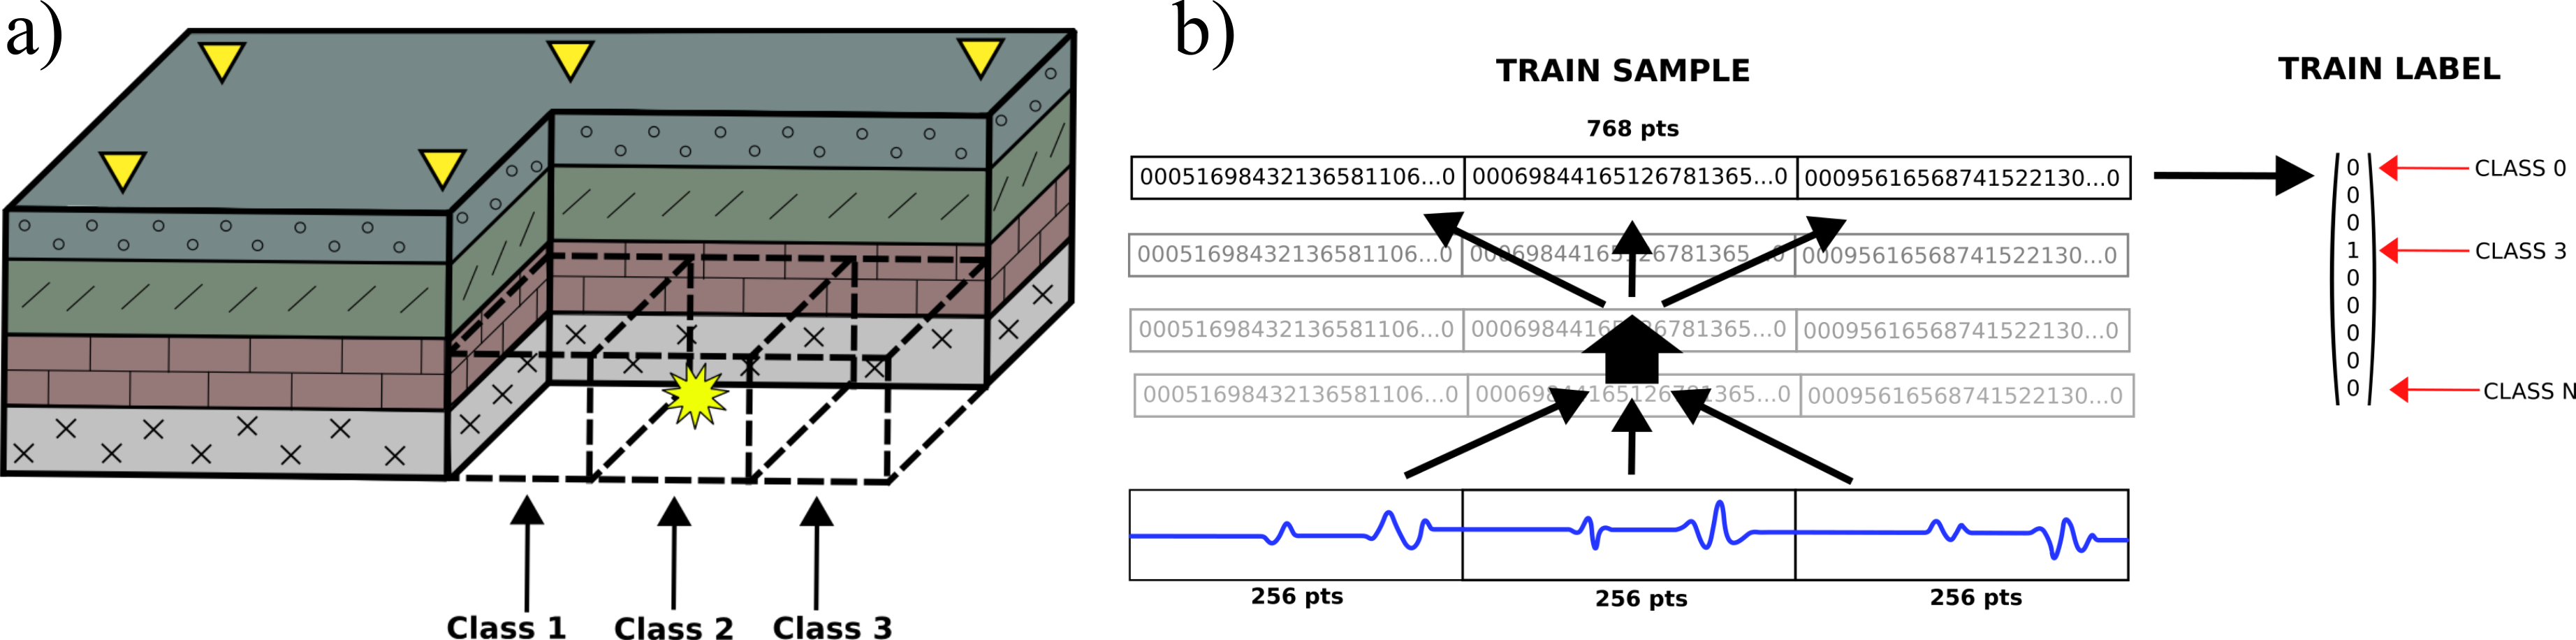
\includegraphics[width=0.7\linewidth,angle=0]{./AntonBiryukov_bibtex/classes.png}
\end{center}
\vspace{-4mm}
\caption{An illustration of the signal classification concept. The signals originating from the locations on the grid (a) are then transformed into a feature space and labeled by the class containing the event origin.}
\label{fig:classes}
\end{figure*}
\begin{itemize}
 \item kurtosis of the signal envelope - to show the peaked-ness of the signal and discern between signals with strong and weak multiple reflections,
 \item mean value of the envelope,
 \item standard deviation of the envelope - to show the variability in the envelope,
 \item area under the envelope,
 \item the ratio of the signal energy contained between $t_{p}$ and $t_{s}$ with respect to the whole trace
 \item number of zero-crossings of the envelope derivative - to count the number of local extrema of the envelope
\end{itemize}
The procedure of modeling and feature extraction is then repeated over the set of values for the moment tensor $M_{i,j}$ and locations covering the range of $2000-5000$ meters.
\subsection*{Signal classification}
\begin{wrapfigure}{r}{0.3\textwidth}
\vspace{-16mm}
\centering
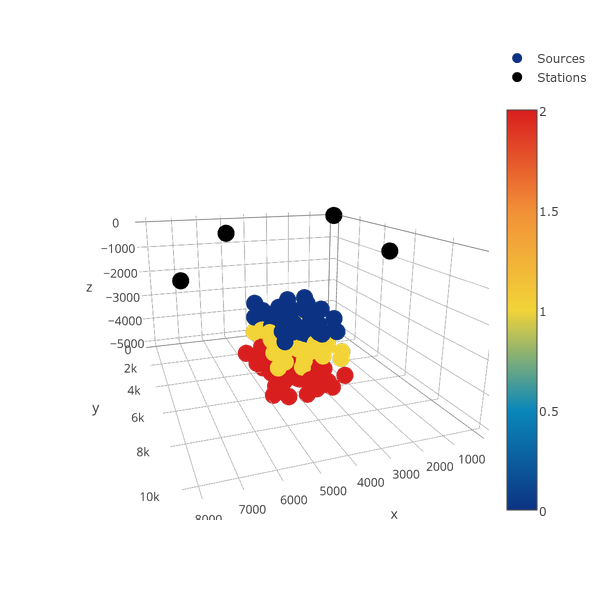
\includegraphics[width=0.28\textwidth]{./AntonBiryukov_bibtex/figure_foxcreek_classes.png}
\vspace{-4mm}
\caption{The relative virtual source-receiver locations for the classification experiment. The colorscale indicates which class an event belongs to.}
\label{fig:foxcreek_classes}
\end{wrapfigure}
The concept of the classification is briefly illustrated in Figure \ref{fig:classes}. The zone of interest is first meshed into nodes that can host virtual sources. The signal from an event originating at a node is transformed into the feature space and is labeled according to the location of the grid. The signal database has been divided into $3$ classes by the origin depth of the event: (i) above \textsc{LVZ}, (ii) within \textsc{LVZ}, and (iii) below \textsc{LVZ}.
The positions were marked according to their relative location with respect to the \textsc{LVZ} as demonstrated in Figure \ref{fig:foxcreek_classes}. For each position of the virtual source $150$ simulations with different values of $M_{i,j}$ were carried out. The database was later split into the training (70\% of the total data) and the test datasets ($30$\% of the total). 
A set of classification algorithms was trained on the training data in order to predict the focal depth of the event (its class) given a set of features of an event of interest from the test data. Therefore, a comparison of prediction accuracy was done between a non-generalizing algorithm - K-nearest-neighbors (\textsc{KNN})~\citep{cover_nearest_1967}, and linear classifiers - logistic regression \citep{jr_applied_2004} and Support Vector Classifier (\textsc{SVC}) with a linear kernel \citep{Guyon93automaticcapacity}. The regularization for the logistic regression and \textsc{SVC}, and the number of neighbors for \textsc{KNN} were tuned through exhaustive grid search over hyperparameter space using 5-fold cross-validation.

Our interpretation here is limited to the analysis of the confusion matrix. The element of the confusion matrix $c_{i,j}$ shows the number of observations from class $i$ predicted into class $j$.


\section*{Results}
\subsection*{Origin uncertainty estimation}
The origin depth uncertainty was estimated for $6$\% velocity perturbation. For both simulations the true location of the event was set to $(X,Y,Z) = (4000,6000,3910)$. The location centroids of MC simulated events for the model are shown Figure \ref{fig:sigma6}. The X and Y coordinates of the event are centered at their true values, whereas the depth of the event shows a bi-modal distribution, with stronger mode centered $240$ meters above the depth. The weaker mode, however tends to center around the true depth of the event.
\evg{the figure is not clear at all}
\begin{figure*}[htb]
\begin{center}
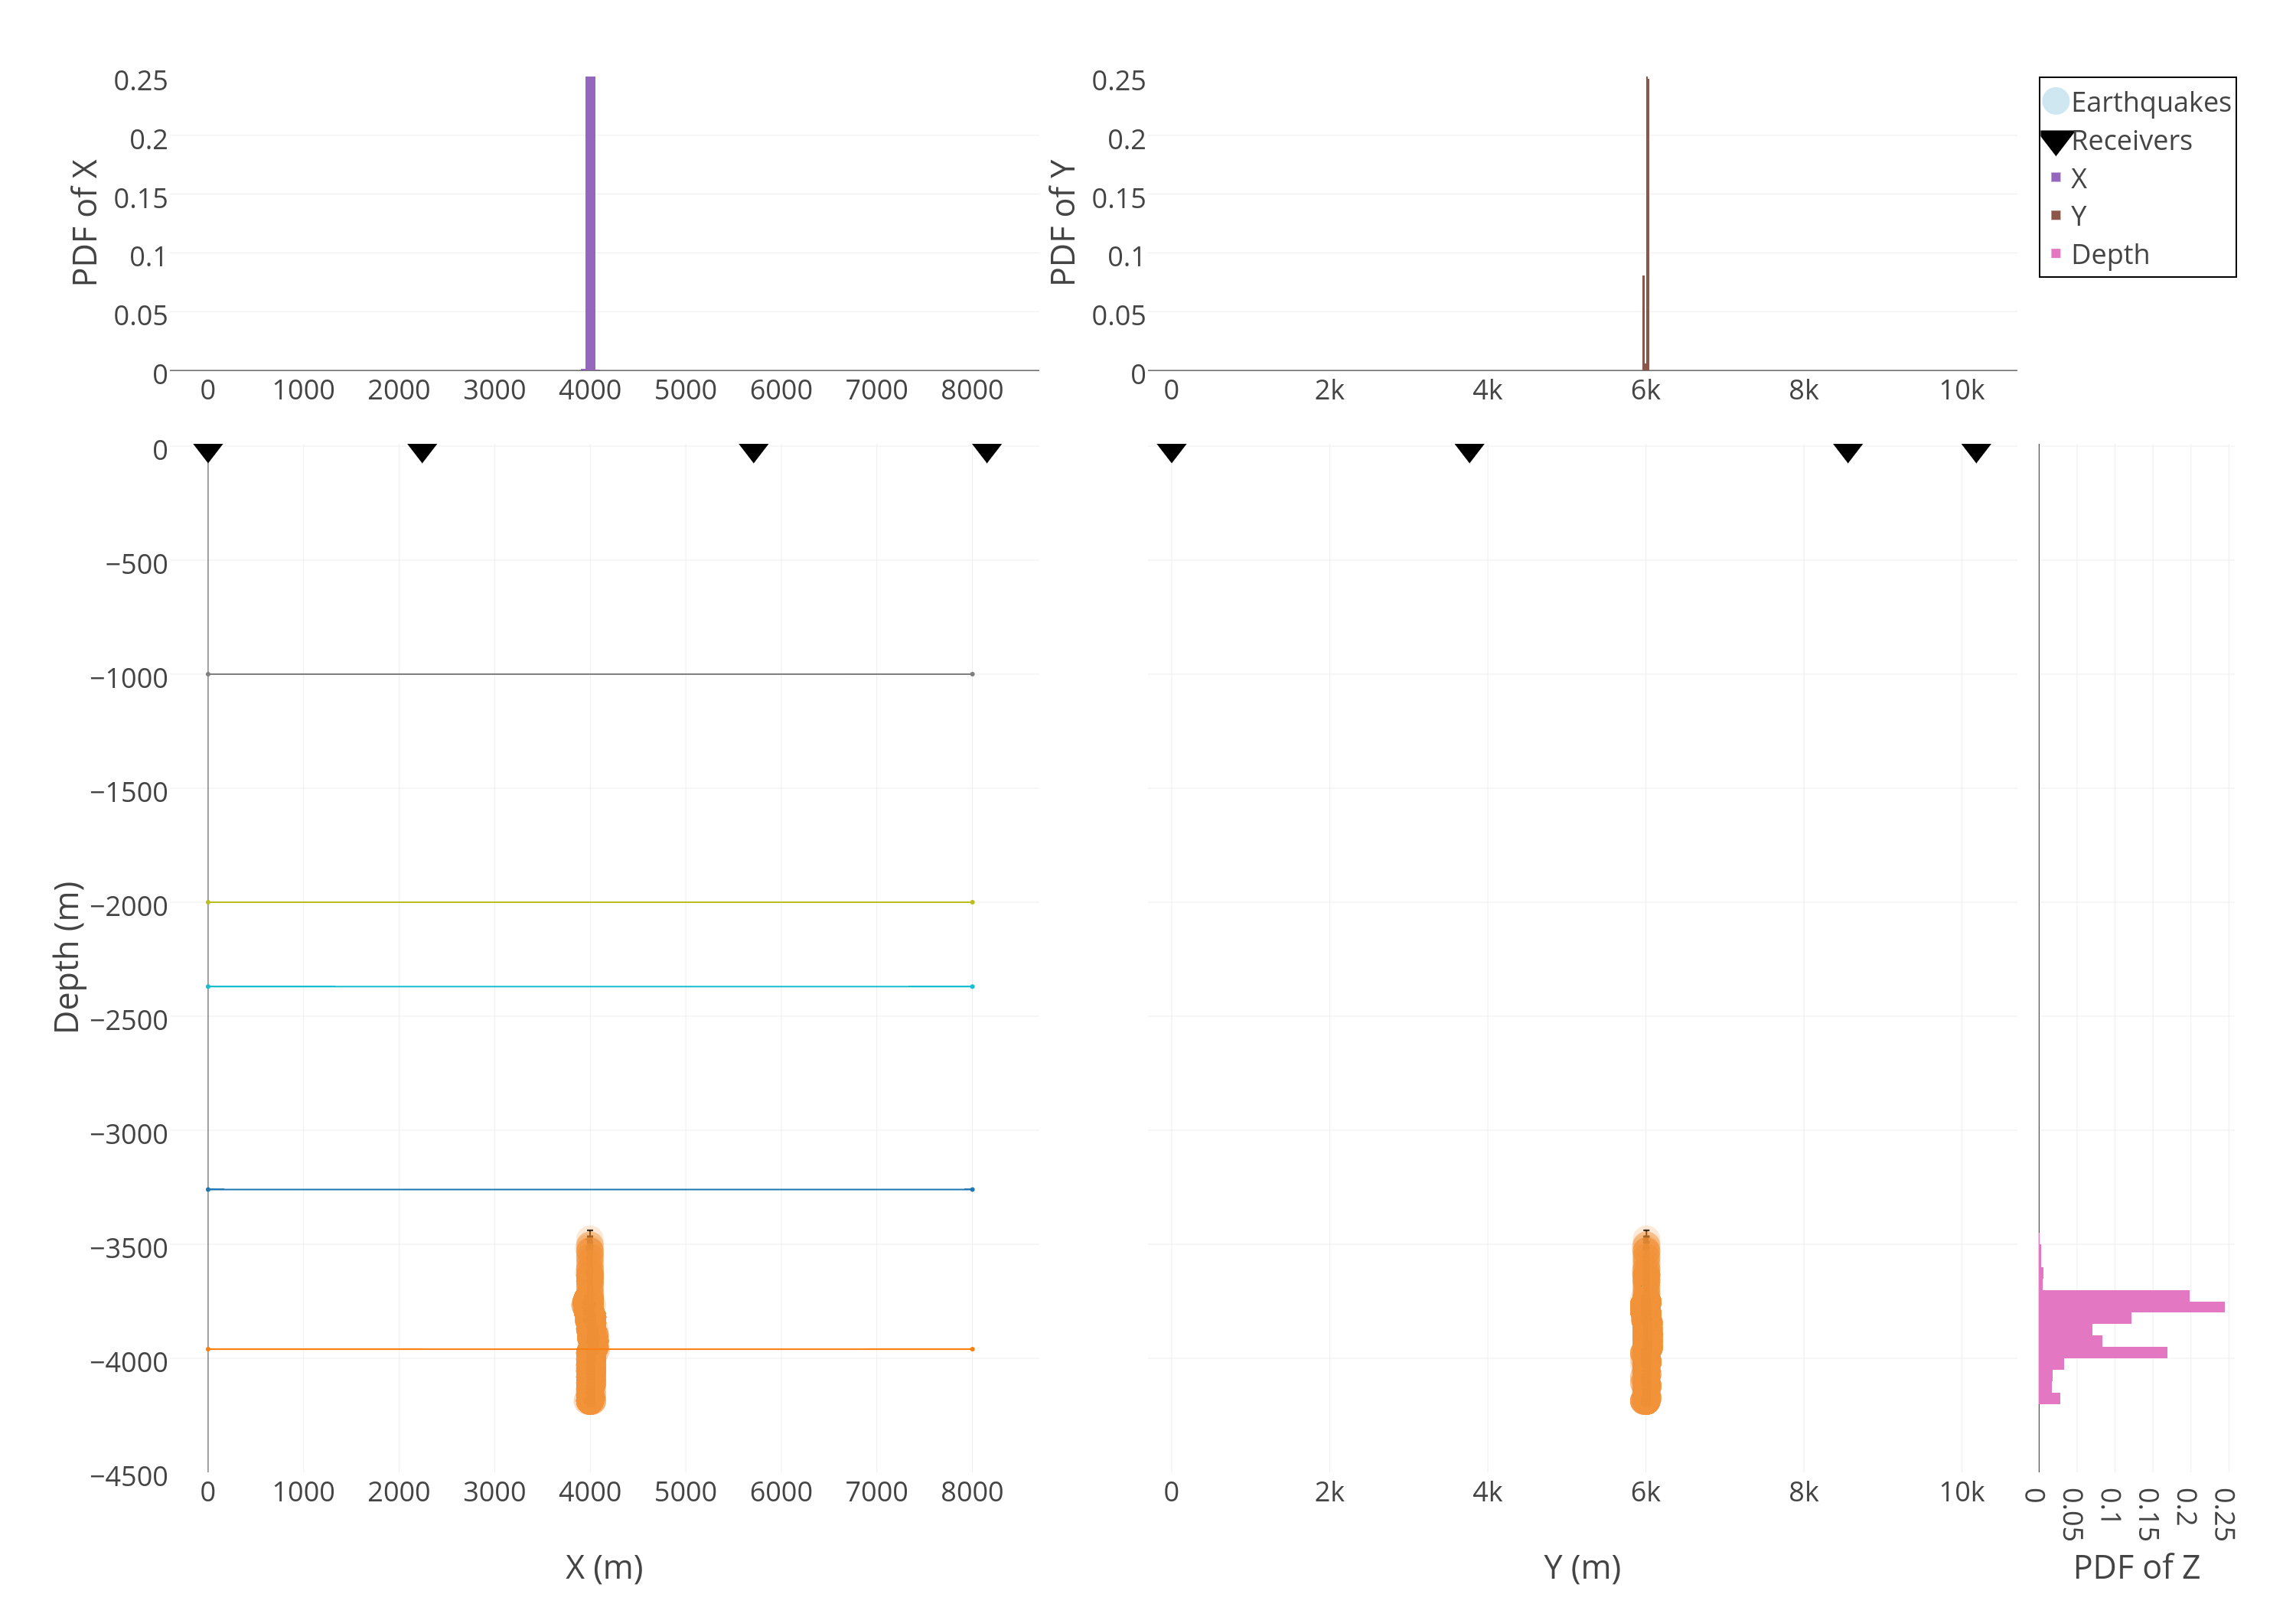
\includegraphics[width=0.6\linewidth,angle=0]{./AntonBiryukov_bibtex/Figure1_6pct.png}
\end{center}
\vspace{-4mm}
\caption{The results of the location of $6$\% velocity perturbation Monte-Carlo simulated virtual events describing the true event at $(X, Y, Z) = (4000, 6000, 3910)$. The receivers are shown in black triangles, the virtual event centroids - in orange circles.}
\label{fig:sigma6}
\end{figure*}
\subsection*{Signal origin classification results}
\begin{wrapfigure}{R}{0.4\textwidth}
\centering
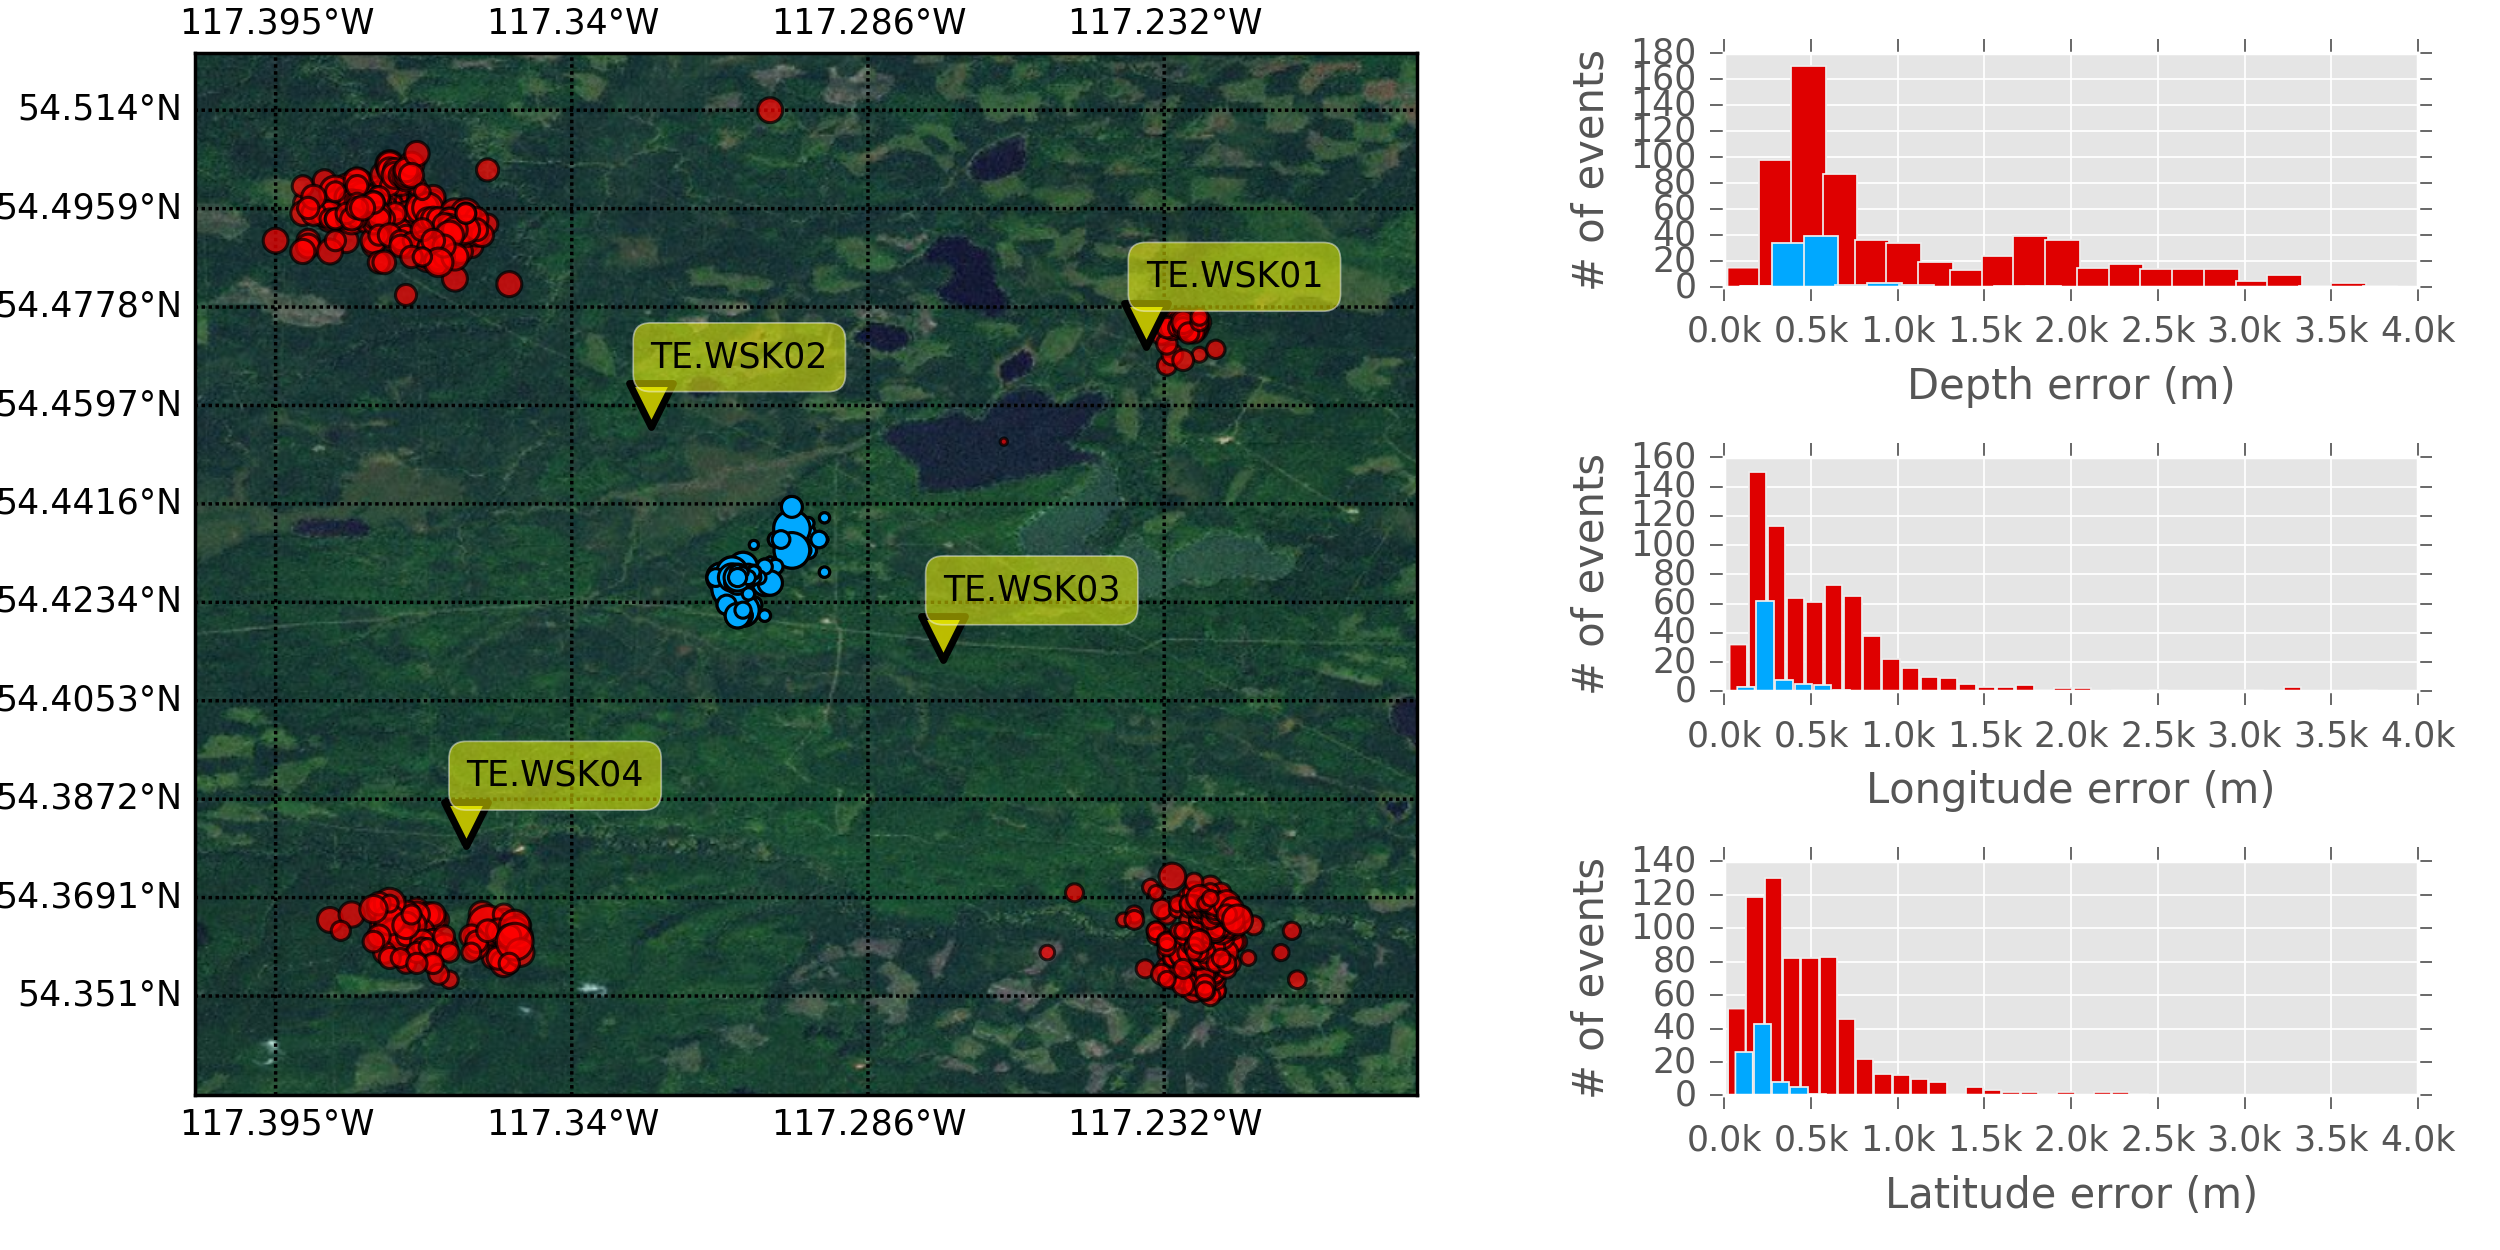
\includegraphics[width=0.38\textwidth]{./AntonBiryukov_bibtex/figure_map_a.png}
\vspace{-4mm}
\caption{The distribution of induced seismicity in Fox Creek area for the events of winter 2015. The central cluster modeled in this study is shown in cyan.}
\label{fig:map_clusters}
\end{wrapfigure}

The classification has been carried out on the database of $90$ different earthquake origins distributed uniformly along the depth range of $2-5$km and covering the area around the central Fox Creek seismicity cluster as shown in Figure \ref{fig:map_clusters}. Here we limit ourselves to a three-class classification based on the proximity of the origin to the \textsc{LVZ} as indicated by the color of the event origin in Figure \ref{fig:foxcreek_classes}.
The classification has been carried out for two feature sets: (A) the travel times for P- and S-phases at each station (a total of $8$ features) and (B) the features from A bundled with the signal features extracted from the vertical channels as described in Methods section. The confusion matrices for the optimally set-up classifiers are shown in Figure \ref{fig:confusion}. One may see that \textsc{KNN} being a non-generalized method shows a better performance compared to \textsc{SVC} and logistic regression for both feature sets ($89$\% vs $85$\% and $86$\% for A, and $98$\% vs $95$\% and $95$\% for B, respectively). The linear classifiers, while exhibiting slightly lower accuracy, are easier to generalize for the future study and do not require storing the dataset in the memory for future application.
%Therefore, the loss in the accuracy might be motivated by the win in the general applicability, which makes both \textsc{SVC} and logistic regression good candidates for the future study.
The accuracy values shown in Figure \ref{fig:confusion} suggest that the added features indeed carry valuable information about the event origin, and consistently contribute towards an increase of in average $10$\% in the accuracy of the classification.
\begin{figure}[htb]
\begin{center}
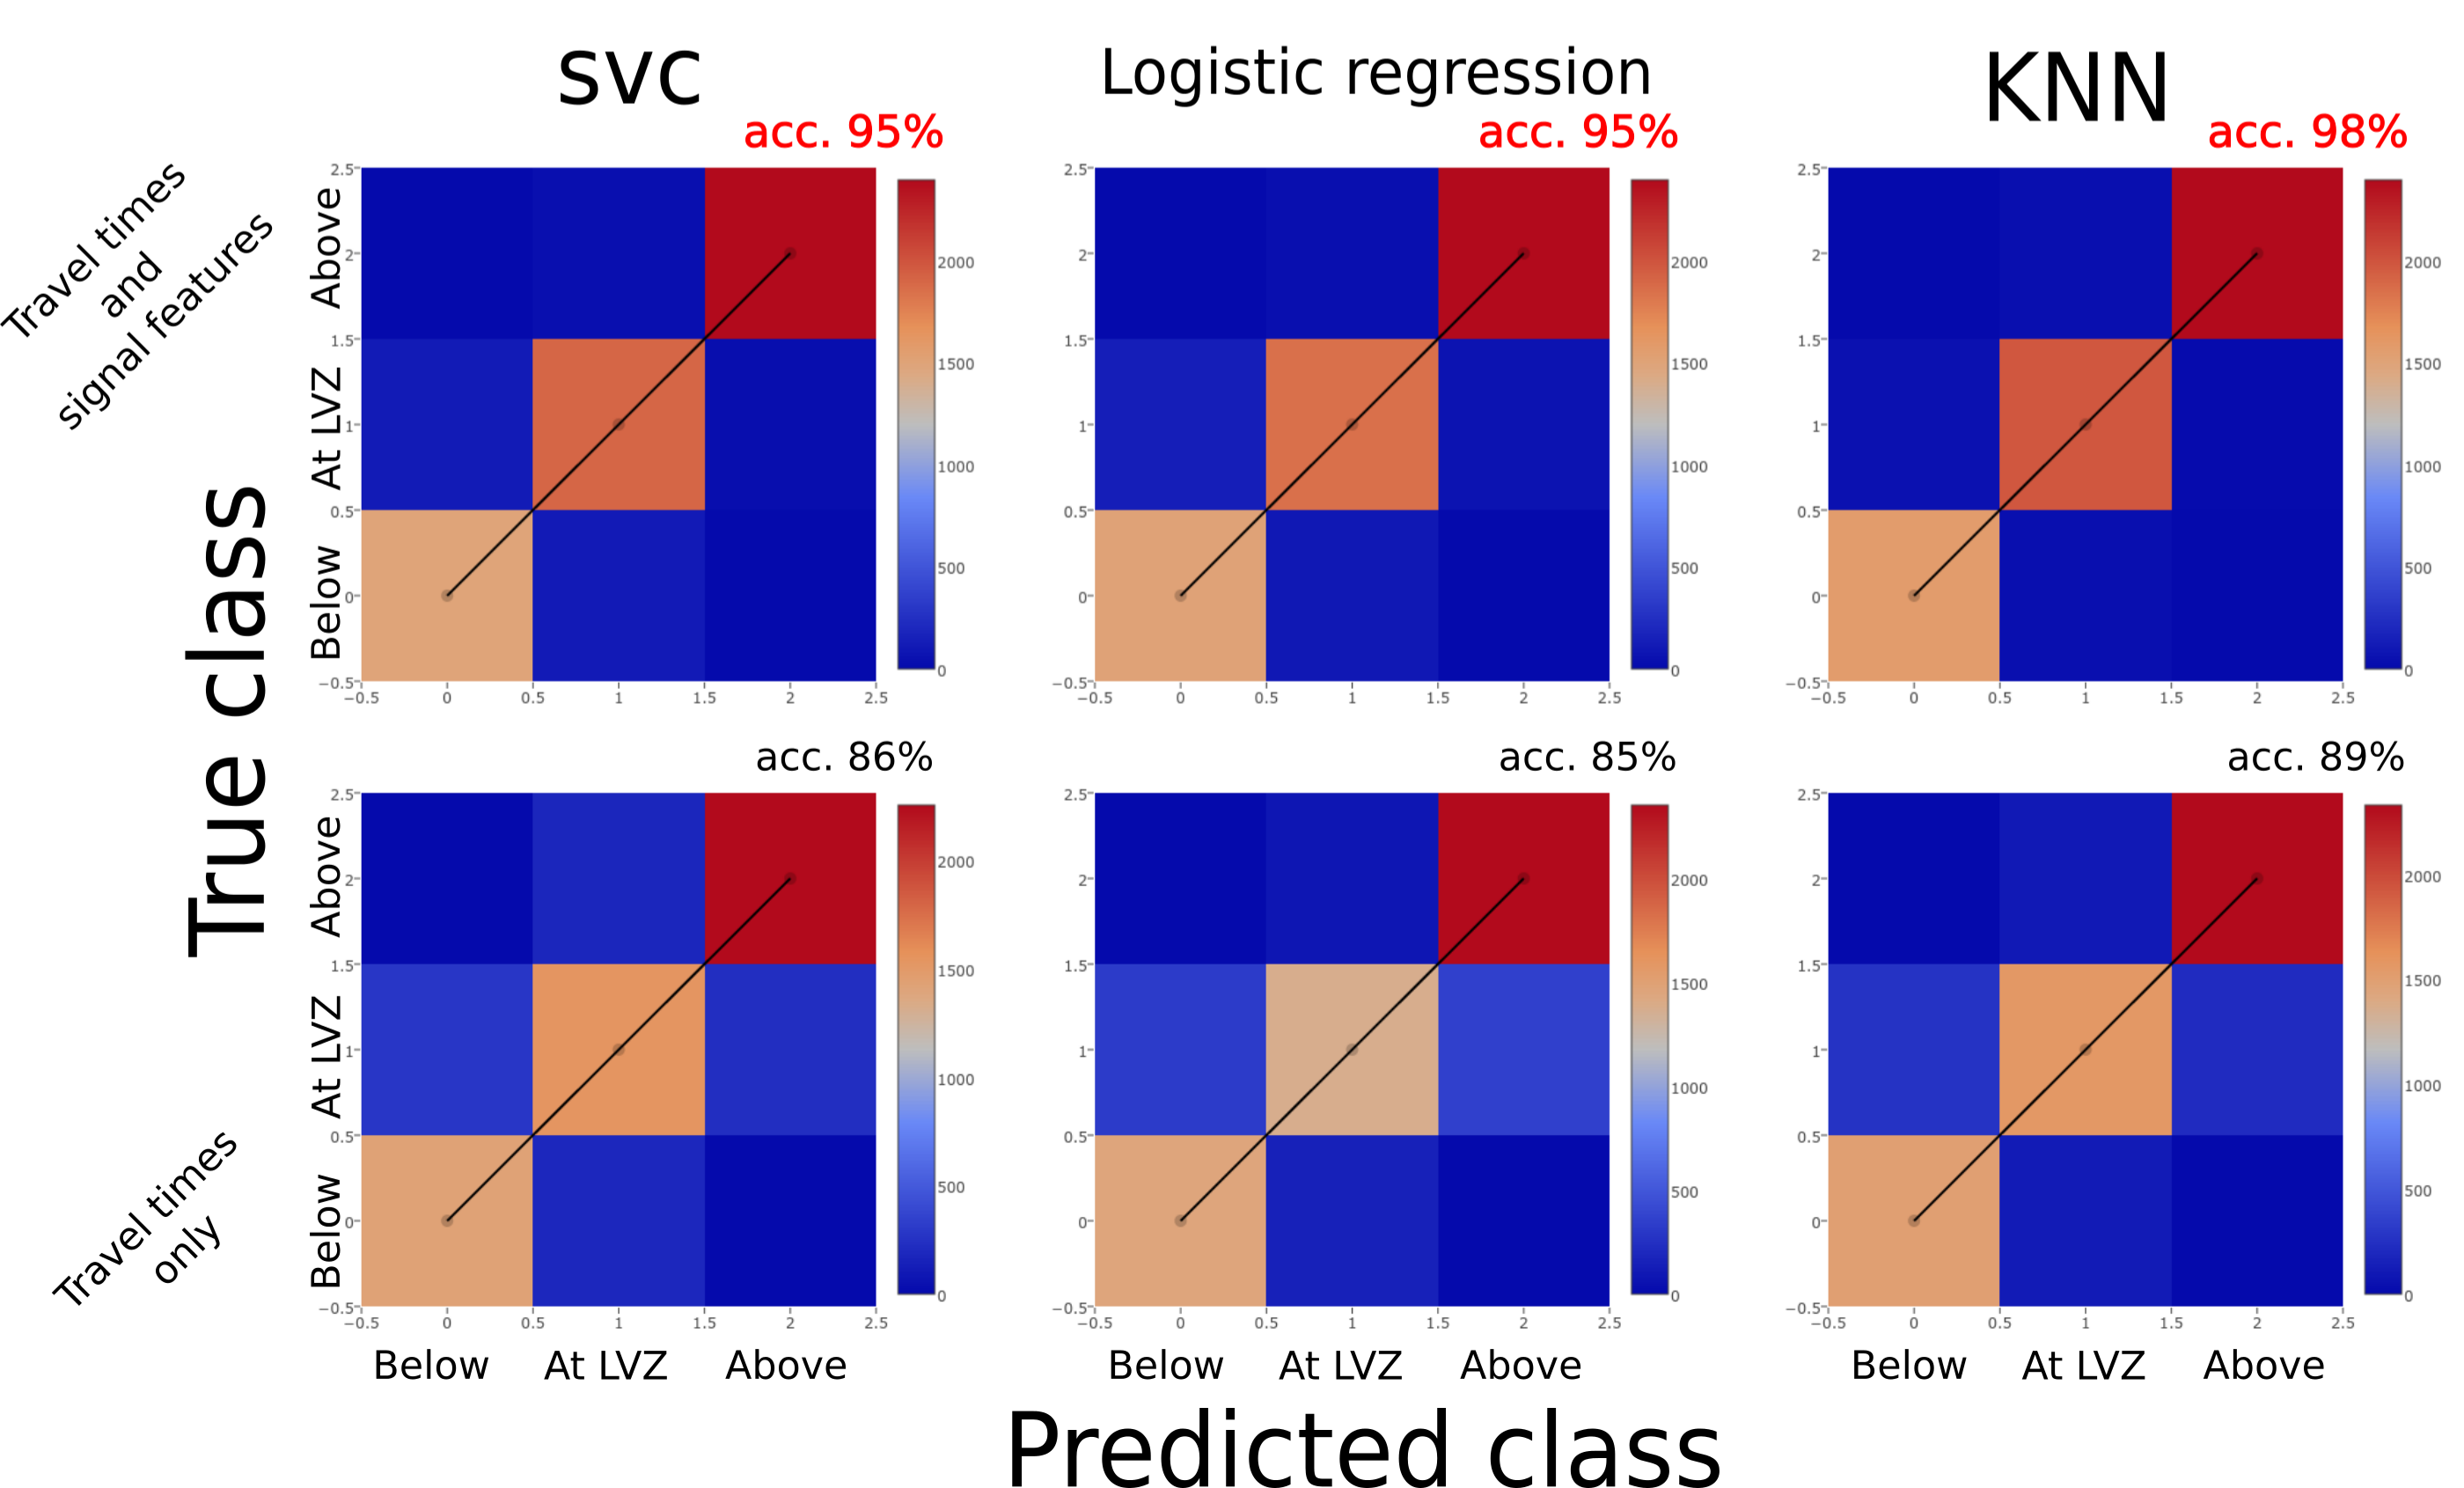
\includegraphics[width=0.5\linewidth,angle=0]{./AntonBiryukov_bibtex/Figure_confusion_horiz.png}
\end{center}
\vspace{-4mm}
\caption{The summary of the classification done with \textsc{KNN}, logistic regression and \textsc{SVC}. The matrices show the proportion between the true and predicted labels on the test dataset.}
\label{fig:confusion}
\end{figure}

\section*{Discussion}
% TO DISCUSSION
As noticed earlier in the Results section, the distribution of the origin depth in the Monte-Carlo simulations shows two distinct modes - $240$ meters above the true origin and at a true origin depth. On one hand, this might be the consequence of the surface acquisition geometry resulting in predominantly near-vertical ray-paths at the surface layer, as opposed to the downhole arrays. On the other hand, it might be caused by the limited and only positive variation allowed for the layer above the \textsc{LVZ} due to the P phase shadowing for farther offset stations. Due to its location with respect to the array, the central cluster is characterized with lower values of horizontal location error compared to other clusters (Figure \ref{fig:map_clusters}). However, as seen from the error distribution, the depth of the location is still poorly constrained for the central cluster and in some cases exceeds $500$ m. Our results from the MC simulations suggest that an error in depth of this magnitude is quite realistic as it reasonably agrees with the predicted depth error for the event at approximately the cluster depth. Therefore, the $6$\% velocity variation within the layers can be a fair estimate of effective velocity model uncertainty when analyzing the effects of the unknown velocity models.
Although we cannot yet provide a solid ground for selecting optimal signal properties, the choice of the particular features is rather logical. The transmitted energy, and interbed multiple arrivals and amplitudes would vary as the function of the event origin. Therefore, it is rational to experiment with the quantities of the signal sensitive to these phenomena. The classification approach demonstrated here is by no means exhaustive, and more work needs to be done in this potentially promising topic.

%It is also important to mention that the location was done here using the grid-search method. The estimates of the uncertainty are likely to change when a different method is used. The choice of the method here was motivated by the presence of a sharp velocity contrast, which often prevents the linearized methods from converging to a global minimum (\citep{lomax_earthquake_2009}).  


%The background velocity model for this study was derived from the sonic log by dividing the measured interval into 6 layers and has not been calibrated. Such a division was based on one person's perception of averaging and layering. While for this particular region, setup and problem it might have been a satisfying approximation, it may not generalize well on the others. Therefore, more attention should be paid towards devising a robust method of velocity profile estimation. One of such methods could be the Reversible Jump Monte-Carlo Markov chain, that could treat the number of layers and values within as unknown and try to fit the step-like function that best explains the variation within the $V_{p}$ or $V_{s}$ log (\citep{sambridge_monte_2002},\citep{bodin_seismic_2009}).


%Given the low values of hypocenter uncertainties, a possible continuation of the work could be towards discretization the depth range and running an N-class classification, where N is the number of classes that would represent possible zones of signal clustering. Alternative route could be relating the signal waveforms to the physics that caused it, e.g. classification between natural earthquakes and mining blasts.


%Finally, the long-term goal of the study is to apply the classification approach to the real data, and combine the real and synthetic datasets together to form a learning database. The success of this combination is based on many factors, including, but not limited to similarity of the synthetics to real data in the feature space, and the accuracy of the ground truth. Therefore, more research needs to be done in choosing the suitable set of signal features. The appropriate feature space would be the one where the real and the synthetic transformed data would have a significant overlap, suggesting that one is likely to represent the other. Devising such a feature space seems challenging, and needs to be addressed in case the inference needs to be done based on very limited real data. The accuracy of the ground truth is also of paramount importance since the lack of it may lead to prediction of erroneous results due to learning from the erroneous data. However, unlike the previous problem, this issue seems tractable in the cases when both downhole and surface seismic data might be available.
%\section*{Conclusions}
%The purpose of this study was two-fold. First we analyzed the effect of the unknown velocity model on the uncertainty of the event origin depth when located using on-surface arrays with limited coverage in Fox Creek area. Our results show that for 6\% uncertainty in the velocity model we may expect up to 800 m of the depth error after the location is performed. The hypocenter of the event shows close to no variation compared to the focal depth variation, as expected given the on-surface acquisition geometry with sufficient azimuthal coverage. The scale of the error implies that the centroid of the event might be placed in two different formations, which can hinder the interpretation and might lead to erroneous conclusions.

%Second, we experimented with several classification methods to determine whether features extracted from the signal can improve the accuracy of our location in a simple framework. We analyzed and compared the results of the classification of the event origin position with respect to the \textsc{LVZ} using travel times only versus travel times and the signal properties extracted from the vertical channels. Our results indicate that in the case of limited acquisition geometry the waveform features can be helpful in improving the accuracy of the origin depth prediction. 
\section*{Acknowledgments}
%
The author would like to thank the sponsors of the Microseismic Industry Consortium for financial support.

\bibliography{./AntonBiryukov_bibtex/bibloSponsors}
\bibliographystyle{plainnat}
\end{document}

